\documentclass[conference]{IEEEtran}

\usepackage{amsmath,amssymb}
\usepackage{booktabs}
\usepackage{cite}
\usepackage{graphicx}
\usepackage{tikz}
\usetikzlibrary{positioning}

\title{ASAP: Adaptive Spherical Anomaly-Guided Purification Against LiDAR Point Cloud Attacks}

\author{
\IEEEauthorblockN{Anonymous Authors}
\IEEEauthorblockA{Paper under double-blind review}
}

\begin{document}
\maketitle

\begin{abstract}
LiDAR-based 3D object detection is a core perception module for autonomous driving, yet point-cloud detectors remain vulnerable to adversarial point injection, perturbation, and dropping. Existing defenses are often detector-specific, require retraining, or denoise the whole scene and remove benign geometry together with adversarial artifacts. We propose ASAP, an Adaptive Spherical Anomaly-Guided Purification framework that protects LiDAR detectors in a detector-agnostic and inference-only manner. ASAP decomposes each scan into density-adaptive spherical purification units, scores their adversarial likelihood with lightweight geometric statistics, and applies a short score-based diffusion purifier only to high-risk units. For sparse off-surface artifacts, an explicitly labeled ASAP-pfilter variant appends a radius-support filter after score-net denoising. Experiments on KITTI and nuScenes with PointPillars, PV-RCNN, VoxelNeXt, and TransFusion-Lidar show that ASAP-family defenses substantially recover detection accuracy without changing detector weights. On nuScenes Perturbation, ASAP-pfilter improves VoxelNeXt from 40.27/51.46 to 52.27/61.23 mAP/NDS and TransFusion-Lidar from 43.02/52.99 to 54.40/61.98, exceeding the strongest ROR baseline on both detectors.
\end{abstract}

\begin{IEEEkeywords}
LiDAR point cloud, 3D object detection, adversarial purification, diffusion model, anomaly detection.
\end{IEEEkeywords}

\section{Introduction}

LiDAR-based 3D object detection is central to autonomous driving perception, supporting downstream prediction, planning, and control \cite{geiger2012kitti,sun2020waymo,caesar2020nuscenes}. Recent work shows that point-cloud detectors are vulnerable to attacks that inject malicious points \cite{cao2019adversarial,tu2020physically}, perturb existing coordinates \cite{xiang2019pointcloud}, or drop selected returns \cite{zheng2019pointcloud}. Since these attacks can transfer across detector architectures, LiDAR robustness requires defenses that are not tied to one detector training recipe.

Existing defenses have practical limitations. Detector-coupled defenses such as adversarial training must be repeated for each architecture \cite{liu2019extending,sun2020towards}. Classical denoisers such as Statistical Outlier Removal (SOR) and Radius Outlier Removal (ROR) \cite{rusu2008towards} are training-free, but apply the same rule across the entire scan and can remove legitimate sparse returns. Diffusion-based purifiers are detector-agnostic \cite{nie2022diffpure,zhang2023ada3diff}, but scene-wide purification is expensive and can smooth benign geometry. LiDAR-SPD \cite{lidarspd} introduces local spherical processing, but uses fixed units and lacks an explicit anomaly gate.

We propose ASAP, an Adaptive Spherical Anomaly-Guided Purification framework. ASAP decomposes a scan into density-adaptive spherical purification units (SPUs), scores each SPU with closed-form geometric statistics, and runs a short VP-SDE purifier only on high-risk units. Low-risk geometry is passed through exactly, and dropping attacks are handled conservatively when evidence has already been removed. Our contributions are:

\begin{itemize}
\item A detector-agnostic, inference-only purification front-end for LiDAR detection.
\item A density-adaptive SPU construction that follows range-dependent LiDAR sampling.
\item An anomaly-selective structure-preservation gate from analytic geometric features and ROC calibration.
\item A two-dataset, four-detector evaluation showing competitive transfer, stronger-than-ROR nuScenes Perturbation recovery with the disclosed pfilter cascade, and clear limitations for dropping.
\end{itemize}

\section{Related Work}

\textbf{LiDAR attacks.} Point-injection attacks place malicious returns to spoof or hide objects \cite{cao2019adversarial,tu2020physically}; point-perturbation attacks shift existing returns within a budget \cite{xiang2019pointcloud,liu2019extending}; and point-dropping attacks remove selected returns \cite{zheng2019pointcloud}. Their transferability motivates detector-agnostic defenses.

\textbf{Point-cloud defenses.} Adversarial training improves robustness by retraining model weights \cite{liu2019extending,sun2020towards}, while certification-oriented approaches such as PointGuard \cite{liu2021pointguard} target point-cloud classification rather than full-scene detection. SOR and ROR \cite{rusu2008towards} are architecture-agnostic, but their global filtering rule does not distinguish malicious points from sparse benign geometry.

\textbf{Diffusion purification.} Diffusion purification projects corrupted inputs back toward the clean data manifold through a short stochastic trajectory \cite{nie2022diffpure,song2021scorebased}. Point-cloud variants include generative diffusion models \cite{luo2021diffusion}, PointDP \cite{sun2023pointdp}, and Ada3Diff \cite{zhang2023ada3diff}. ASAP differs by operating locally, adaptively, and selectively, so the score network is invoked only for anomalous SPUs.

\section{ASAP Framework}

Let $P=\{p_i\}_{i=1}^{N}\subset\mathbb{R}^3$ be an input LiDAR scan and $\mathcal{D}$ an off-the-shelf detector. ASAP returns a purified scan $\hat P$ with the same point-cloud format, then invokes $\mathcal{D}(\hat P)$ without detector retraining.

\begin{figure}[t]
\centering
\small
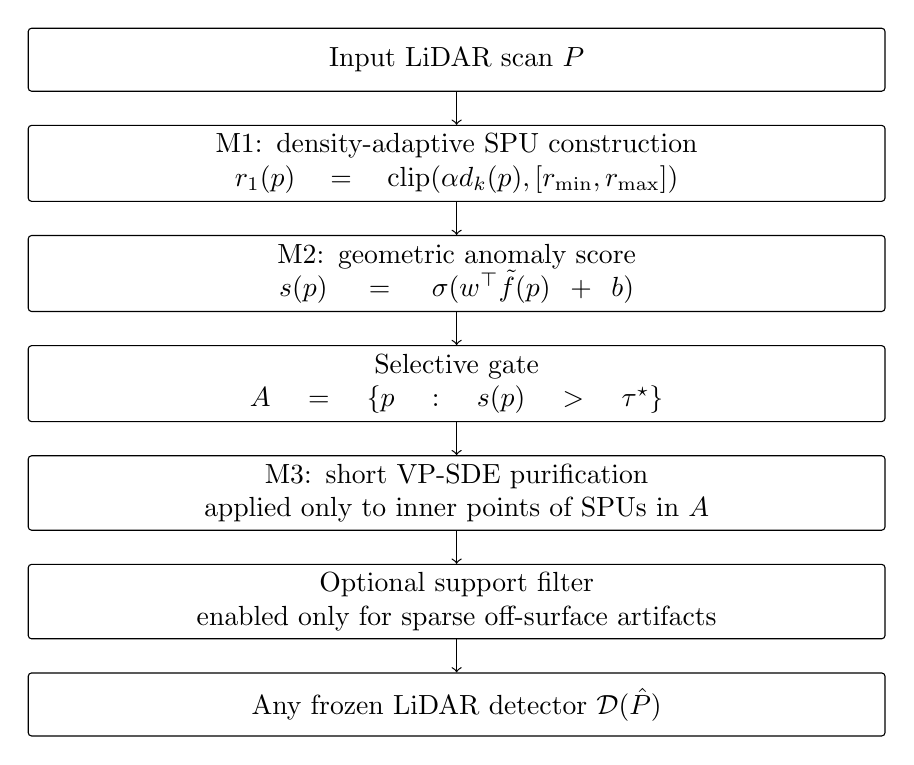
\begin{tikzpicture}[
  node distance=4.2mm,
  block/.style={
    draw,
    rounded corners=1.2pt,
    align=center,
    minimum height=8mm,
    text width=0.88\linewidth,
    inner sep=3pt
  },
  arrow/.style={->, line width=0.45pt}
]
\node[block] (input) {Input LiDAR scan $P$};
\node[block, below=of input] (m1) {M1: density-adaptive SPU construction\\
$r_1(p)=\mathrm{clip}(\alpha d_k(p),[r_{\min},r_{\max}])$};
\node[block, below=of m1] (m2) {M2: geometric anomaly score\\
$s(p)=\sigma(w^\top \tilde f(p)+b)$};
\node[block, below=of m2] (gate) {Selective gate\\
$A=\{p:s(p)>\tau^\star\}$};
\node[block, below=of gate] (m3) {M3: short VP-SDE purification\\
applied only to inner points of SPUs in $A$};
\node[block, below=of m3] (filter) {Optional support filter\\
enabled only for sparse off-surface artifacts};
\node[block, below=of filter] (det) {Any frozen LiDAR detector $\mathcal{D}(\hat P)$};
\draw[arrow] (input) -- (m1);
\draw[arrow] (m1) -- (m2);
\draw[arrow] (m2) -- (gate);
\draw[arrow] (gate) -- (m3);
\draw[arrow] (m3) -- (filter);
\draw[arrow] (filter) -- (det);
\end{tikzpicture}
\caption{ASAP is an inference-only front-end. It builds density-adaptive spherical purification units, scores them with detector-agnostic geometric features, purifies only high-risk local regions, and optionally applies a disclosed support filter for sparse artifacts. The downstream detector is kept frozen.}
\label{fig:asap_pipeline}
\end{figure}


\subsection{Adaptive SPU Construction}

For a candidate center $p$, let $d_k(p)$ be the distance to its $k$-th nearest neighbor. We define
\begin{equation}
r_1(p)=\mathrm{clip}\!\left(\alpha d_k(p),[r_{\min},r_{\max}]\right),\qquad
r_2(p)=\beta r_1(p),
\end{equation}
where $r_1$ is the outer SPU radius and $r_2$ is the editable inner radius. Candidate centers are sampled by farthest point sampling. The full SPU is $\mathcal{S}(p)=\{q\in P:\|q-p\|_2\le r_1(p)\}$, with inner points $P_{\mathrm{in}}(p)=\{q\in P:\|q-p\|_2\le r_2(p)\}$ and annulus points $P_{\mathrm{an}}(p)=\mathcal{S}(p)\setminus P_{\mathrm{in}}(p)$. We use $\alpha=2$, $k=16$, $\beta=0.67$, $r_{\min}=0.10$m, and $r_{\max}=0.40$m.

\subsection{Anomaly-Selective Structure Gate}

M2 summarizes each SPU with four detector-agnostic geometric statistics: compactness $f_c=|P_{\mathrm{in}}|/V_2$, PCA anisotropy $f_a=1-\lambda_3/(\lambda_1+\lambda_2+\lambda_3)$, vMF concentration $f_v=\hat{\kappa}$ using the approximation of Banerjee et al. \cite{banerjee2005clustering}, and density ratio $f_d=(|P_{\mathrm{in}}|/V_2)/(|P_{\mathrm{an}}|/V_{\mathrm{an}}+\varepsilon)$. After standardizing each feature with clean-set statistics, ASAP computes
\begin{equation}
s(p)=\sigma\!\left(w_c\tilde f_c+w_a\tilde f_a+w_v\tilde f_v+w_d\tilde f_d+b\right),
\end{equation}
where the five parameters are fitted by logistic regression on held-out SPUs. The operating threshold is selected by Youden's index \cite{youden1950index},
\begin{equation}
\tau^\star=\arg\max_\tau \mathrm{TPR}(\tau)-\mathrm{FPR}(\tau).
\end{equation}
This gate is not merely a compute shortcut: SPUs below threshold are never edited, preserving benign local structure.

\subsection{Selective Score-Based Purification}

For each anomalous SPU $p$ with $s(p)>\tau^\star$, ASAP centers and rescales $X_p=\mathrm{stack}(P_{\mathrm{in}}(p))$ into $\tilde X_p=(X_p-p)/r_2(p)$, applies a short forward-then-reverse VP-SDE trajectory \cite{song2021scorebased}, and maps the result back to metric space. Overlapping edits are averaged per original point; untouched points remain exactly unchanged.

For sparse off-surface artifacts, ASAP-pfilter additionally retains a point $\hat q$ only if it has at least $m_f$ neighbors within radius $r_f$. The pfilter rows are therefore a score-net plus support-filter cascade, not a pure diffusion row. We compare them directly against ROR using the same support rule on the attacked input.

\section{Experiments}

\subsection{Setup}

KITTI \cite{geiger2012kitti} is used for controlled ablations with PointPillars \cite{lang2019pointpillars} and PV-RCNN \cite{shi2020pvrcnn}. nuScenes \cite{caesar2020nuscenes} is used for detector-transfer evaluation with VoxelNeXt \cite{chen2023voxelnext} and TransFusion-Lidar \cite{bai2022transfusion}. KITTI reports Car/Moderate AP$_{R40}$ and cross-class mAP. nuScenes reports mAP and NDS. On nuScenes, attacks edit only the current keyframe while OpenPCDet still loads clean historical sweeps; Dropping is excluded because its attack-strength gate failed under this protocol.

\begin{table*}[t]
\centering
\scriptsize
\setlength{\tabcolsep}{3.2pt}
\caption{Main robustness results. KITTI cells report Car/Moderate AP$_{R40}$ / cross-class mAP. nuScenes cells report mAP / NDS. ASAP-v1 denotes the M1/M2-gated score-net purifier without the optional support filter. ASAP-pfilter denotes the explicitly disclosed score-net + support-filter cascade. nuScenes attacks edit only the current keyframe while OpenPCDet still loads clean historical sweeps; Dropping is excluded from nuScenes main rows because its keyframe-only attack-strength gate failed.}
\label{tab:main_results}
\begin{tabular}{llllrrrr}
\toprule
Dataset & Detector & Family & Attack & Clean & No defense & Best non-ASAP & ASAP family \\
\midrule
KITTI & PointPillars & pillar & Injection & 78.40/64.21 & 60.10/38.73 & 66.07/51.30 ROR & 65.71/\textbf{52.18} \\
KITTI & PointPillars & pillar & Perturb. & 78.40/64.21 & 56.54/27.32 & 41.65/19.46 ROR & \textbf{61.04/34.69} \\
KITTI & PointPillars & pillar & Dropping & 78.40/64.21 & 71.22/48.42 & 49.91/34.20 ROR & \textbf{71.22/48.42} \\
KITTI & PV-RCNN & voxel-point & Injection & 84.36/69.74 & 63.16/48.22 & \textbf{72.77/57.77} ROR & 72.59/57.73 \\
KITTI & PV-RCNN & voxel-point & Perturb. & 84.36/69.74 & 3.50/2.45 & 1.94/1.17 ROR & \textbf{10.96/5.98} \\
KITTI & PV-RCNN & voxel-point & Dropping & 84.36/69.74 & 78.61/57.12 & 59.05/43.12 ROR & \textbf{78.61/57.12} \\
nuScenes & VoxelNeXt & sparse voxel & Injection & 60.52/66.64 & 21.97/41.87 & \textbf{53.29/62.66} ROR & 52.45/62.18 \\
nuScenes & VoxelNeXt & sparse voxel & Perturb. & 60.52/66.64 & 40.27/51.46 & 51.36/60.40 ROR & \textbf{52.27/61.23} pfilter \\
nuScenes & TransFusion-L & query head & Injection & 64.57/69.43 & 19.13/39.45 & \textbf{57.29/65.04} ROR & 56.74/64.72 \\
nuScenes & TransFusion-L & query head & Perturb. & 64.57/69.43 & 43.02/52.99 & 53.51/61.23 ROR & \textbf{54.40/61.98} pfilter \\
\bottomrule
\end{tabular}
\end{table*}

\begin{table}[t]
\centering
\scriptsize
\setlength{\tabcolsep}{3.5pt}
\caption{Policy and innovation ablations supporting the final attack-aware ASAP family. Results are reported as mAP / NDS for nuScenes and Car/Moderate AP$_{R40}$ / cross-class mAP for KITTI.}
\label{tab:policy_ablations}
\begin{tabular}{llrl}
\toprule
Setting & Detector / attack & Result & Takeaway \\
\midrule
No defense & PointPillars / Perturb. & 56.54/27.32 & Attacked lower bound \\
Fixed-SPU all-unit diffusion & PointPillars / Perturb. & 57.16/30.35 & Heavy nonselective proxy \\
Adaptive-SPU all-unit diffusion & PointPillars / Perturb. & 38.62/17.88 & Over-purification collapse \\
ASAP Track A & PointPillars / Perturb. & \textbf{61.04/34.69} & Adaptive selective purification wins \\
No defense & VoxelNeXt / Perturb. & 40.27/51.46 & Strong accepted budget \\
ASAP-v1 & VoxelNeXt / Perturb. & 41.32/52.74 & Score-net alone is insufficient \\
ROR / support-only & VoxelNeXt / Perturb. & 51.36/60.40 & Strong classical baseline \\
ASAP-pfilter & VoxelNeXt / Perturb. & \textbf{52.27/61.23} & +0.91 mAP over support-only \\
ROR / support-only & TransFusion-L / Perturb. & 53.51/61.23 & Transfer baseline \\
ASAP-pfilter & TransFusion-L / Perturb. & \textbf{54.40/61.98} & +0.89 mAP over support-only \\
Score-net policy & PointPillars / Dropping & 68.49/35.41 & Extra editing removes evidence \\
Skip M3 & PointPillars / Dropping & \textbf{71.22/48.42} & Conservative policy is safer \\
\bottomrule
\end{tabular}
\end{table}

\begin{table}[t]
\centering
\scriptsize
\setlength{\tabcolsep}{3.5pt}
\caption{Preprocessing selectivity and throughput for representative ASAP policies. SPU and point columns are percentages. Throughput is estimated from completed two-shard T4 pipeline logs and excludes detector inference.}
\label{tab:cost_selectivity}
\begin{tabular}{lrrrr}
\toprule
Setting & Flagged SPUs & Score SPUs & Point edit/drop & ms/frame \\
\midrule
KITTI Injection & 13.55 & 9.71 & 1.96 / 5.02 & 529 \\
KITTI Perturb. & 28.26 & 24.45 & 21.91 / 0.00 & 764 \\
KITTI fixed-SPU all-unit Perturb. & 100.00 & 97.14 & 77.86 / 0.00 & 2390 \\
KITTI adaptive-SPU all-unit Perturb. & 100.00 & 95.92 & 70.98 / 0.00 & 3623 \\
nuScenes Injection & 21.76 & 17.76 & 4.19 / 17.74 & 483 \\
nuScenes Perturb. pfilter & 22.75 & 18.87 & 4.78 / 16.63 & 482 \\
\bottomrule
\end{tabular}
\end{table}


\subsection{Main Results}

Table~\ref{tab:main_results} shows that ASAP-family defenses recover substantial accuracy without modifying detector weights. Injection recovery is near ROR rather than uniformly above it: ROR remains slightly higher on PV-RCNN and both nuScenes Injection rows. Perturbation is the strongest setting for ASAP: on KITTI PointPillars, ASAP Track A improves cross-class mAP from 27.32 to 34.69, while ROR drops to 19.46. On nuScenes Perturbation, ASAP-pfilter exceeds ROR on both VoxelNeXt and TransFusion-Lidar. Dropping is handled conservatively by skipping M3; the paper does not claim point restoration when object evidence has already been removed.

\subsection{Ablations and Cost}

Table~\ref{tab:policy_ablations} isolates the main design choices. A fixed-SPU all-unit diffusion proxy reaches 57.16/30.35 on KITTI PointPillars Perturbation, below ASAP Track A at 61.04/34.69 while editing 77.86\% of points. Keeping adaptive SPUs but removing M2 selection collapses to 38.62/17.88, showing that M2 is a structure-preservation gate rather than only a runtime filter. Stricter thresholds also fail to improve the final policy: increasing $\tau$ from 0.024 to 0.036 and 0.048 reduces mAP from 34.69 to 30.21 and 28.79.

Table~\ref{tab:cost_selectivity} reports preprocessing selectivity. The current prototype is slower than ROR, but it is detector-agnostic and does not require retraining. On nuScenes Perturbation pfilter, 22.75\% of candidate SPUs are flagged, 18.87\% enter the score-net path, 4.78\% of points are coordinate-edited, and the support filter removes 16.63\% of points.

\section{Conclusion}

ASAP is an inference-only LiDAR purification framework built from density-adaptive SPUs, an anomaly-selective structure gate, and local score-based purification with an optional support filter for sparse artifacts. Experiments across KITTI and nuScenes show detector transfer, near-ROR Injection recovery, and stronger-than-ROR nuScenes Perturbation recovery when the disclosed pfilter cascade is enabled. ASAP does not reconstruct evidence removed by strong dropping attacks; under the current keyframe-only nuScenes protocol, dropping remains outside the main robustness claim. Future work includes adaptive attacks aware of ASAP's gate, density-drop reconstruction, and extension to multi-modal detectors.

\bibliographystyle{IEEEtran}
\bibliography{references}

\end{document}
